
\begin{frame}{Theoretical Background}{Basic aerodynamics and airfoil theory}
	1D momentum theory:
	\begin{itemize}
		\item Air slows down due to delivery of energy from air to rotor blades
		\item Air expands due to conservation of mass
	\end{itemize}

	\begin{figure}[ht]
		\centering
		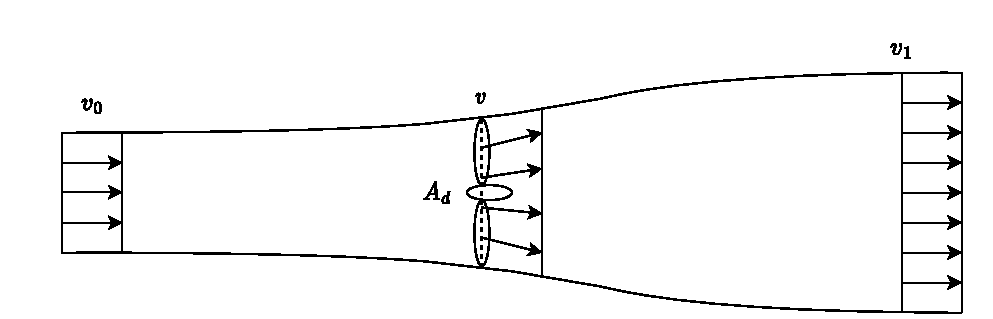
\includegraphics[width=1\linewidth]{../Graphics/FlowThroughRotor.pdf}
		\label{fig:betz}
	\end{figure}
\end{frame}

%%%%%%%%%%%%%%%%%%

\begin{frame}{Theoretical Background}{Basic aerodynamics and airfoil theory}
	Power of wind moving through rotor:
	\begin{equation} \label{eq:power}
		P_{air} = \dfrac{1}{2} \dot{m} \, v_0^2 = \dfrac{1}{2}\rho \, A_d v_0^3
	\end{equation}
	
	Extractable power defined by \textit{power coefficient} $ C_p $:
	\begin{equation}\label{eq:power_w_Cp}
		P_{T} = \dfrac{1}{2} \rho \, A_d v_0^3 C_p(\theta, \lambda)
	\end{equation}
	where $ \lambda $ is the tip-speed ratio (TSR):
	\begin{equation}\label{key}
		\lambda = \dfrac{R \Omega}{v_0}
	\end{equation}
	The theoretically highest achievable $ C_p $ is the \textit{betz limit}:
	\begin{equation}\label{eq:betzlimit}
		C_{pbetz} = 0.5962
	\end{equation}
	The optimal $ C_p $ for a given turbine is achieved at specific TSR and $ \theta $:
	\begin{equation}\label{eq:cp_optimal}
		C_p^\star = C_p(\theta^\star, \lambda^\star)
	\end{equation}
\end{frame}

%%%%%%%%%%%%%%%%%%

\begin{frame}{Theoretical Background}{Blade element theory}
	\begin{itemize}
		\item Forces are calculated on blade sections (b)
		\item Thrust and torque calculated from velocity triangle (a)
	\end{itemize}
	
	\begin{figure}[ht]
		\centering
		\subfloat[Blade cross section]{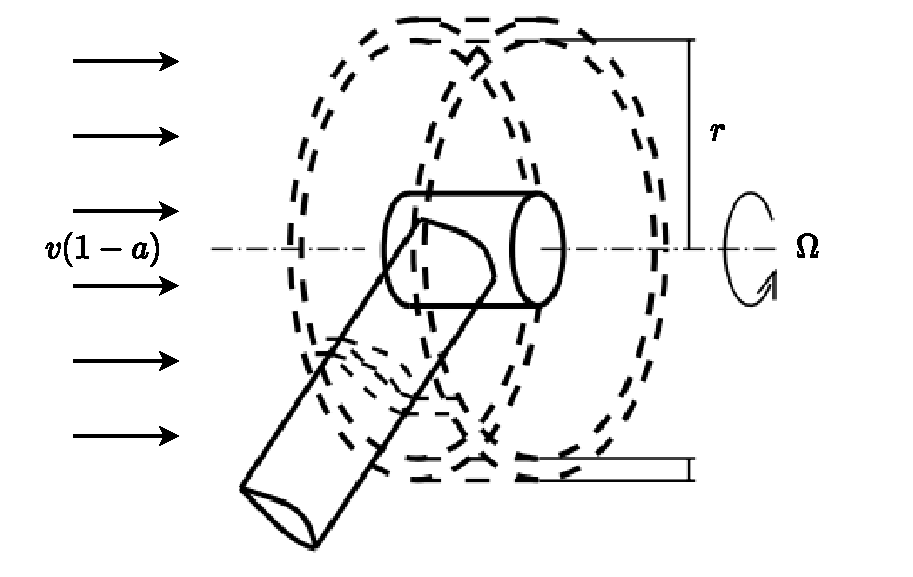
\includegraphics[width=.44\textwidth]{../Graphics/RotorBladeElement.pdf}%
			\label{fig:blade_vel_triangles}}
		\hfil
		\subfloat[Velocity triangle]{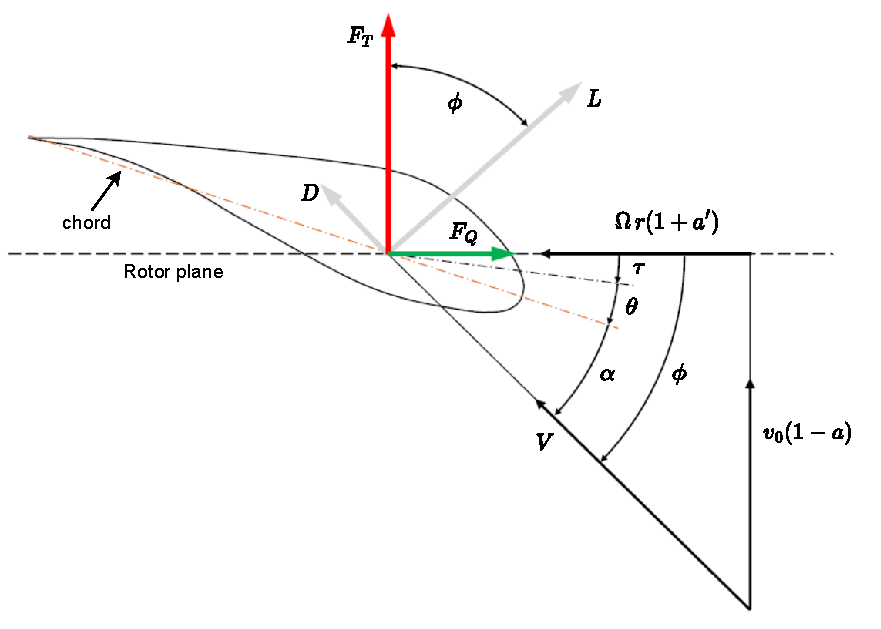
\includegraphics[width=.55\textwidth]{../Graphics/BladeVelocityTriangle.pdf}%
			\label{fig:blade_vel_triangle}}
		\label{fig:blade_triangles}
	\end{figure}
\end{frame}

%%%%%%%%%%%%%%%%%%

\begin{frame}{Theoretical Background}{Something}
	\begin{itemize}
		\item A text in a dotted list in the theoretical background
	\end{itemize}
\end{frame}

%%%%%%%%%%%%%%%%%%





%%%%%%%%%%%%%%%%%%
%\begin{frame}{Big header}{Smaller header}
%	\textbf{Some text}
%	\begin{itemize}
%		\item Item
%	\end{itemize}
%\end{frame}
%
